\documentclass[pdflatex,sn-nature]{sn-jnl}
\usepackage{graphicx}
\usepackage{amsmath,amssymb}
\usepackage{booktabs}
\usepackage{array}
\usepackage{xcolor}
\usepackage{placeins}
\raggedbottom
\usepackage{url}
\setlength{\emergencystretch}{3em}
\hypersetup{hidelinks}
\begin{document}
\title{Reusability report: Tabular foundation models for cancer survival prediction from multiomics}
\author*[1]{\fnm{Vatsal P.} \sur{Patel}}\email{vatsal1@hawkfranklin.in}
\author[1]{\fnm{Satya Prakash} \sur{Mohanty}}
\affil[1]{\orgname{HawkFranklin Research}, \orgaddress{\country{India}}}
\abstract{Tabular foundation models make predictions from a labeled table in a single forward pass, and TabPFN was introduced as giving accurate predictions on small datasets without task-specific tuning. Clinical cohorts are small tables, which makes these models attractive for cancer research. Here we assess the reusability of TabPFN, together with its later generations and Google's TabFM, first on its own benchmark data and then on survival prediction from cancer multiomics. On six of its benchmark datasets, TabPFN again had the highest mean ROC AUC among default-setting models (0.877 against 0.873 for CatBoost), a directional reproduction under a simpler protocol than the original, and five TabPFN generations and TabFM differed by less than 0.01. We then evaluated eleven models on 3,238 patients from five TCGA and CPTAC cancer cohorts using 400 frozen test sets. Within single cancers, survival prediction was difficult for every model and no two nonlinear models differed significantly. Pooling the cancers raised ROC AUC to 0.721 for 3-year survival ($n = 1{,}645$) and 0.786 for extreme survival ($n = 937$), but tree ensembles matched these scores and controls using only cancer type or the pattern of zero-valued features reached similar levels. Scored within each cancer, pooled training lowered the ROC AUC of TabFM by 0.084 and TabPFN v3 by 0.070 at 5 years, losses that were larger on average than those of tree ensembles. TabPFN ran without tuning and performed comparably to default tree ensembles on single-cancer survival tasks, but pooled pan-cancer scores should be reported with within-cancer results and shortcut controls.}
\keywords{tabular foundation models; TabPFN; TabFM; reusability; cancer multiomics; survival prediction; cohort shortcuts}
\maketitle
\raggedbottom

\section*{Introduction}

For most of the history of machine learning on tables, the honest recommendation has been gradient-boosted trees. Random forests, XGBoost, LightGBM, CatBoost and AutoML systems built on them handle mixed feature scales, missing values and nonlinear interactions with little tuning, and careful benchmarks have repeatedly found that deep networks struggle to beat them on medium-sized tabular data with many more rows than features.\citep{breiman2001random,chen2016xgboost,ke2017lightgbm,prokhorenkova2018catboost,erickson2020autogluon,grinsztajn2022tree}

Hollmann and colleagues challenged that recommendation with TabPFN, described in their title as giving ``accurate predictions on small data with a tabular foundation model''.\citep{hollmann2025accurate} TabPFN is a transformer pretrained on synthetic tables; at prediction time it reads the labeled training rows as context and returns predictions without fitting task-specific parameters. On 29 classification and 28 regression datasets of up to 10,000 rows and 500 features, the original study reported that it outperformed gradient-boosted baselines both at default settings and after up to four hours of tuning, taking seconds per dataset on a machine with a GPU. Later releases extended the supported data size, to 50,000 rows and 2,000 features for TabPFN-2.5 and to larger regimes for TabPFN-3,\citep{priorlabs2025tabpfn25,priorlabs2026tabpfn3} and Google's TabFM, described in an announcement and a software release, applies the same in-context principle with row-and-column attention and a synthetic prior built from structural causal models.\citep{google2026tabfm,tabfmsoftware2026} An independent comparison against tuned established methods on twelve binary clinical tasks found that TabPFN exceeded the best of them in 2 of 12 tasks, with most differences in AUROC within 0.02, although with predictors, endpoints and budgets that differ from ours.\citep{shaktah2026established}

Cancer multiomics is a natural, and demanding, place to reuse these models. Cohorts typically contain a few hundred patients and thousands of molecular features. Benchmarks of censored survival models on TCGA cohorts have found that a clinical-variables-only reference performs about as well as the best molecular models in aggregate, and that adding modalities does not reliably help.\citep{herrmann2021benchmark,li2024combining,wissel2023systematic} Cohorts also differ in prognosis, source and assay coverage, and TCGA molecular profiles are organized largely by cell of origin,\citep{hoadley2018cell} so differences between cancers are biological as well as technical. When several cohorts are harmonized into one table, these differences can become features: a model may recognize the cohort and predict its average outcome, a shortcut that can score well under random cross-validation and transfer poorly.\citep{soneson2014batch,bernau2014crossstudy,geirhos2020shortcut}

In this report we first reproduce TabPFN on datasets from its original benchmark and compare its generations with TabFM. We then evaluate four TabPFN generations, TabFM, AutoGluon and five classical learners on survival classification within five cancer cohorts, using identical frozen patient splits. Third, we pool the cancers and test the resulting gain against controls that contain no patient-level biology. Finally, we ask whether pooled training helps or harms prediction among patients who share a diagnosis (Fig.~\ref{fig:roadmap}). Our own early single-split analyses had read the pooled gain as a shared prognostic signal; the last two steps are how we tested that reading.

\begin{figure}[t]
\centering
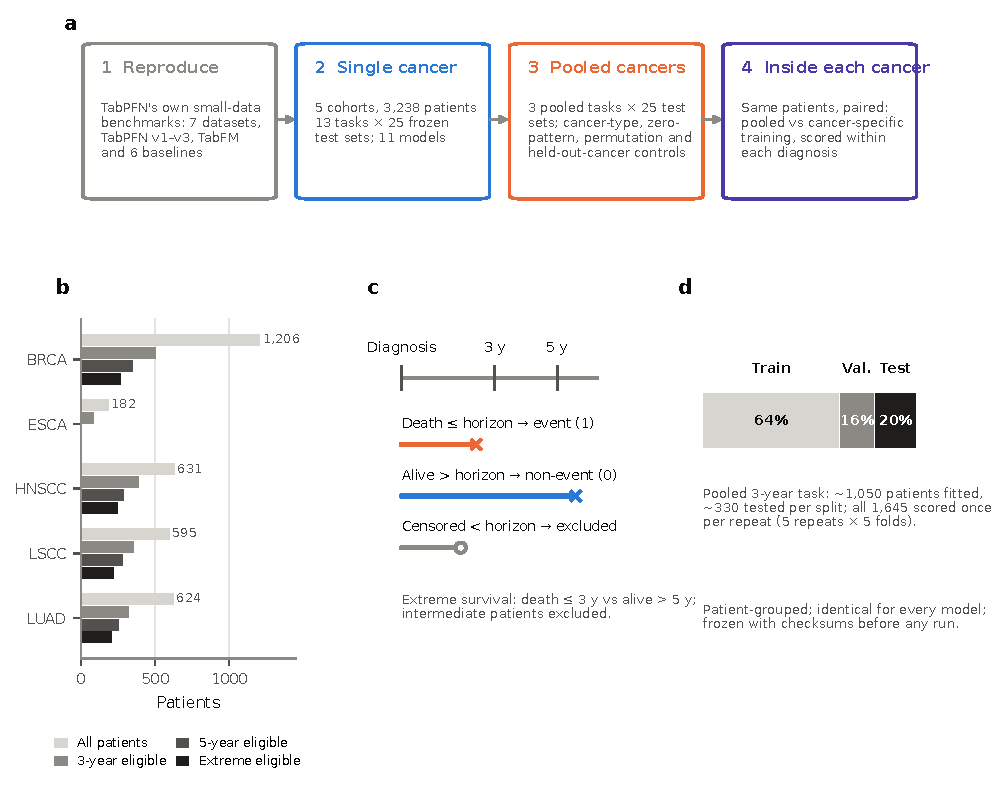
\includegraphics[width=\linewidth,height=0.64\textheight,keepaspectratio]{figures/reusability/fig1_roadmap_and_design.pdf}
\caption{\textbf{Study roadmap and evaluation design.} \textbf{a}, The four steps of the report: reproduction of TabPFN on its own benchmark datasets, evaluation within single cancers, evaluation on the pooled cancers with shortcut controls, and a paired return to within-cancer scoring. \textbf{b}, Patients per cohort: all patients (lightest bar) and those eligible for 3-year survival, 5-year survival and extreme survival (progressively darker bars); the number gives the cohort total. ESCA was too small to form the 5-year and extreme-survival endpoints. \textbf{c}, Fixed-horizon labels: death on or before the horizon is an event (1), follow-up beyond the horizon is a non-event (0), and patients censored before the horizon are excluded; extreme survival compares death within 3 years with survival beyond 5 years. \textbf{d}, Partition of patients in one frozen test set: about 64\% for training, where features are selected; 16\% for validation, used only to choose the decision threshold; and 20\% for testing, scored once. Splits are patient-grouped, identical for every model and frozen before any run.}
\label{fig:roadmap}
\end{figure}

\section*{Reproducibility}

Hollmann and colleagues evaluated TabPFN on 29 classification and 28 regression datasets with up to 10,000 rows, 500 features and 10 classes, using ten seeds with a 90/10 train/test split, baselines tuned by random search for between 30 seconds and four hours, scores normalised within each dataset (best method 1, worst 0), and a GPU for TabPFN.\citep{hollmann2025accurate} We did not repeat that protocol. We re-ran TabPFN on seven of its classification datasets (ada, australian, blood-transfusion, car, churn, cmc and credit-g), reporting raw ROC AUC on one stratified split per dataset that held out 15\% of rows, and compared TabPFN with CatBoost, XGBoost, LightGBM, random forest, logistic regression and AutoGluon, all without hyperparameter tuning. Baseline runs for ada did not complete, leaving six datasets for the comparison.

The direction of the central claim reproduced (Fig.~\ref{fig:reproduction}a,b). TabPFN had the highest mean test ROC AUC, 0.877, followed by CatBoost at 0.873, XGBoost at 0.863 and AutoGluon at 0.861; logistic regression reached 0.797. TabPFN was best or tied for best on four of six datasets, second on credit-g and fourth on churn. These raw ROC AUC values are not comparable with the original's normalised scores, which were 0.939 for default TabPFN and 0.752 for default CatBoost on classification.\citep{hollmann2025accurate} With six datasets and one split each, and baselines that were not tuned, our margins confirm the direction of the original finding and not its size.

We then compared generations under a common protocol with training sets capped at 1,024 rows (Fig.~\ref{fig:reproduction}c). On the six datasets where every model completed (TabPFN v3 failed on ada in this run), mean ROC AUC was 0.856 for TabPFN v1, 0.862 for v2, 0.863 for v2.5, 0.857 for v2.6, 0.861 for v3 and 0.859 for TabFM. On small public benchmarks, then, successive generations and an independently developed foundation model behave almost interchangeably. Rankings in large benchmarks depend on tuning budgets, validation design and ensembling,\citep{erickson2025tabarena,qu2025tabicl} so we compare generations only under this one protocol and do not rank them in general.

\begin{figure}[t]
\centering
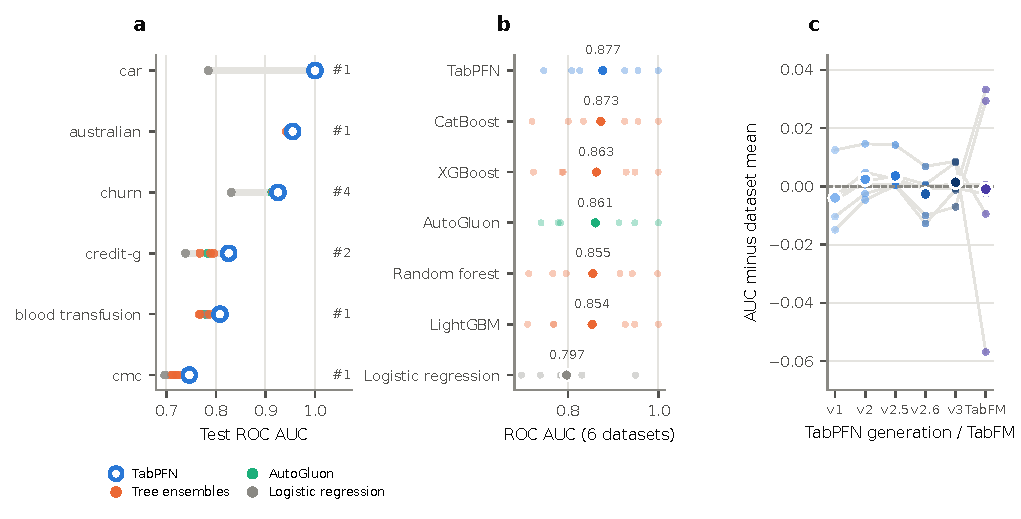
\includegraphics[width=\linewidth,height=0.64\textheight,keepaspectratio]{figures/reusability/fig2_reproduction.pdf}
\caption{\textbf{The direction of TabPFN's benchmark advantage reproduces on its own datasets.} \textbf{a}, TabPFN against six baselines: test ROC AUC of TabPFN (open circle) and of tree ensembles, AutoGluon and logistic regression (filled points) on six benchmark datasets. The grey bar spans the baselines, and the number on the right is TabPFN's rank on that dataset (ties share a rank). \textbf{b}, Mean test ROC AUC of each model over the six datasets (large point, value above) with per-dataset values (small points). \textbf{c}, Four TabPFN generations and TabFM under a common protocol with training capped at 1,024 rows: ROC AUC relative to each dataset's mean across these six models (lines join datasets; large points are means). Mean ROC AUC over the six datasets was 0.856 (v1), 0.862 (v2), 0.863 (v2.5), 0.857 (v2.6), 0.861 (v3) and 0.859 (TabFM). One stratified split per dataset.}
\label{fig:reproduction}
\end{figure}

\section*{Reusability}

\subsection*{Five cancer cohorts and 400 frozen test sets}

We combined breast invasive carcinoma (BRCA), esophageal carcinoma (ESCA), head and neck squamous cell carcinoma (HNSCC), lung squamous cell carcinoma (LSCC) and lung adenocarcinoma (LUAD) from TCGA and CPTAC, 3,238 patients in total (Fig.~\ref{fig:roadmap}b and Table~\ref{tab:cohorts}).\citep{tcga2012brca,tcga2017esca,tcga2015hnsc,tcga2012lusc,tcga2014luad,liu2018clinical,li2023pancancer} The original TCGA marker papers profiled fewer tumours than these cohorts contain (825 breast, 164 oesophageal, 279 head and neck, 178 squamous lung and 230 lung adenocarcinomas),\citep{tcga2012brca,tcga2017esca,tcga2015hnsc,tcga2012lusc,tcga2014luad} so our counts reflect the later PanCancer Atlas and CPTAC data and not those publications. The cohorts are also internally heterogeneous: the oesophageal cohort spans histological subtypes and the head and neck cohort spans HPV-positive and HPV-negative tumours from different anatomical sites.\citep{tcga2017esca,tcga2015hnsc} Patients censored before a horizon cannot be labeled, which left 1,645 patients for 3-year survival, 1,168 for 5-year survival and 937 for an exploratory extreme-survival endpoint that compares death within 3 years with survival beyond 5 years (Fig.~\ref{fig:roadmap}c).

This defines 16 prediction tasks: 13 cancer-specific tasks and three pooled endpoints. Each was split into five repeats of five patient-grouped folds, and the resulting 400 test sets were frozen before any model was run. In the pooled 3-year task, each model was fitted on about 1,050 patients and tested on about 330 per split (Fig.~\ref{fig:roadmap}d). Cancer-specific test sets were much smaller, usually fewer than 70 patients.

\begin{table}[ht]
\centering
\caption{Cancer cohort size and endpoint eligibility. Extreme survival contrasts death within 3 years against survival beyond 5 years. NA, endpoint-specific cohort not formed.}
\label{tab:cohorts}
\begin{tabular}{lrrrr}
\toprule
Cohort & Raw & 3-year eligible & 5-year eligible & Extreme eligible \\
\midrule
BRCA & 1206 & 501 & 350 & 268 \\
ESCA & 182 & 86 & NA & NA \\
HNSCC & 631 & 385 & 286 & 244 \\
LSCC & 595 & 355 & 281 & 222 \\
LUAD & 624 & 318 & 251 & 203 \\
\bottomrule
\end{tabular}

\end{table}

\subsection*{Within a single cancer, no model wins decisively}

Modeled one cancer at a time, survival was hard for every method (Fig.~\ref{fig:within}a). A foundation model had the highest mean ROC AUC in 7 of the 13 tasks, sometimes by a useful margin: in breast cancer extreme survival, TabPFN v2.6 reached 0.613 against 0.569 for the best classical model. Where foundation models trailed, they trailed by at most 0.024. Fold-matched differences from random forest were centered near zero for every nonlinear model (Fig.~\ref{fig:within}b).

Ranked across the 13 tasks, TabPFN v2.5 had the best mean rank (4.8), followed by TabPFN v2 (5.1) and random forest (5.2; Fig.~\ref{fig:within}c). The models differed overall (Friedman $\chi^2 = 20.3$, $P = 0.026$), but the difference came from logistic regression (mean rank 9.4). No two of the ten nonlinear models differed by more than the Nemenyi critical difference of 4.19 ranks.\citep{demsar2006statistical} In this setting TabPFN is reusable: it installs and runs without tuning and performed comparably to default-setting tree ensembles. A non-significant difference is not evidence of equivalence, and with cancer-specific test sets of usually fewer than 70 patients these comparisons could resolve only large differences. TabPFN is not, however, a clear improvement over the tree ensembles. Averaged over endpoints, the within-cancer ROC AUC was 0.568 for TabPFN v2.5, 0.565 for TabFM and 0.561 for random forest (Table~\ref{tab:model_auc}).

\begin{figure}[tbp]
\centering
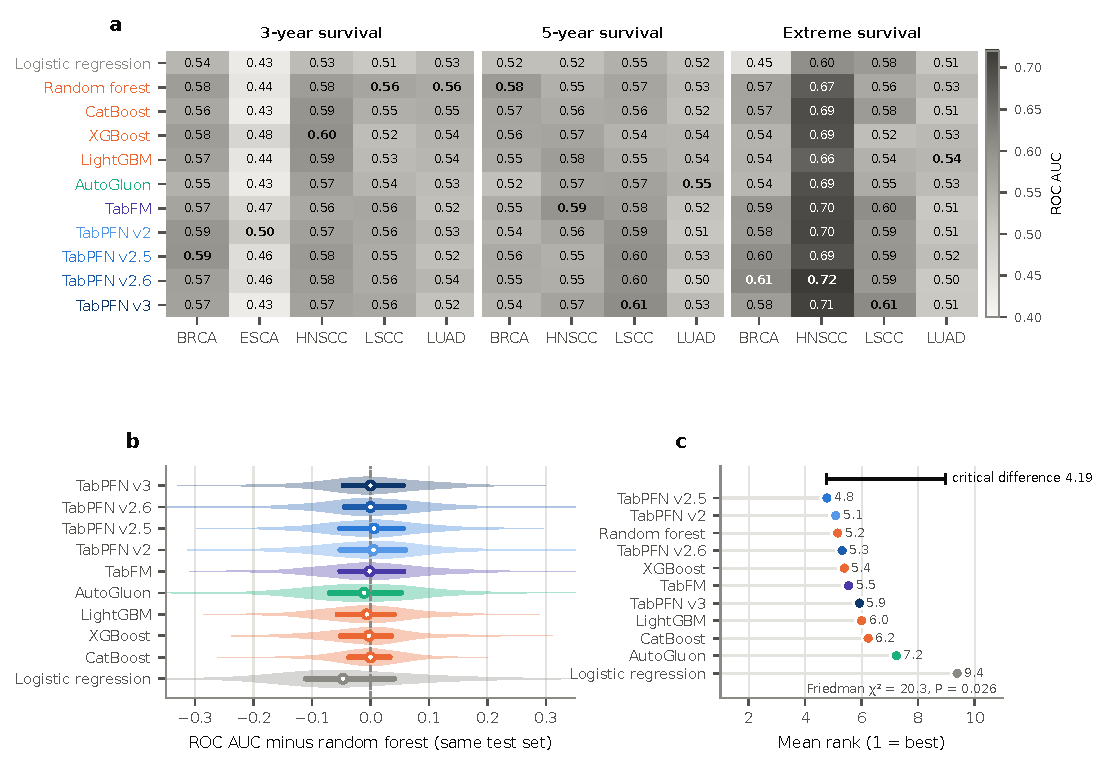
\includegraphics[width=\linewidth,height=0.64\textheight,keepaspectratio]{figures/reusability/fig3_within_cancer.pdf}
\caption{\textbf{Within a single cancer, no model wins decisively.} \textbf{a}, ROC AUC in each of the 13 cancer-specific tasks, grouped by endpoint (3-year, 5-year and extreme survival); each cell is the mean over 25 frozen test sets, and bold marks the best model in each column. \textbf{b}, Paired difference from random forest: distribution of fold-matched ROC AUC differences over the 325 cancer-specific test sets (violin), with interquartile range (bar) and median (circle); the dashed line marks no difference. \textbf{c}, Mean rank of each model across the 13 tasks (1 = best). The bar shows the Nemenyi critical difference at $\alpha = 0.05$; models whose mean ranks differ by less than this are not significantly different. Model names are coloured by family.}
\label{fig:within}
\end{figure}

\subsection*{Pooling lifts every capable model}

Training on all cancers together changed the picture abruptly (Fig.~\ref{fig:pooling}a). For 3-year survival, TabFM reached a mean ROC AUC of 0.721 and TabPFN v3 0.714, while random forest reached 0.716 and CatBoost 0.713. For 5-year survival, TabPFN v3 reached 0.754 against 0.749 for CatBoost, and for extreme survival 0.786 against 0.782. Every nonlinear model gained between 0.14 and 0.22 over its within-cancer level. Logistic regression, restricted to a linear function of the selected features, did not (0.536 at 3 years).

Taken at face value this is the result that motivates pan-cancer modeling. Two features of it argue for caution. The gain was the same size for in-context foundation models, boosted trees and AutoML, more than would be expected from a capacity only some architectures have. And the largest values occurred for extreme survival, which removes the patients with intermediate outcomes and is therefore an easier question rather than a better answer to the fixed-horizon one.

\begin{table}[ht]
\centering
\caption{Mean ROC AUC across frozen test sets. Within-cancer is the average of the three endpoint summaries, each itself averaged over cancers. NA, pooled 3-year training sets exceeded the 1,000-sample CPU limit of TabPFN v2--v2.6.}
\label{tab:model_auc}
\footnotesize\setlength{\tabcolsep}{3pt}\begin{tabular}{llrrrr}
\toprule
Model & Family & Within-cancer & Pooled 3-year & Pooled 5-year & Pooled extreme \\
\midrule
Logistic regression & Linear & 0.524 & 0.536 & 0.542 & 0.522 \\
Random forest & Tree ensemble & 0.561 & 0.716 & 0.747 & 0.781 \\
CatBoost & Boosted tree & 0.559 & 0.713 & 0.749 & 0.782 \\
XGBoost & Boosted tree & 0.556 & 0.701 & 0.734 & 0.768 \\
LightGBM & Boosted tree & 0.554 & 0.698 & 0.719 & 0.762 \\
AutoGluon & AutoML & 0.550 & 0.702 & 0.744 & 0.757 \\
TabFM & Foundation model & 0.565 & 0.721 & 0.753 & 0.780 \\
TabPFN v2 & Foundation model & 0.567 & NA & 0.751 & 0.784 \\
TabPFN v2.5 & Foundation model & 0.568 & NA & 0.753 & 0.785 \\
TabPFN v2.6 & Foundation model & 0.566 & NA & 0.752 & 0.778 \\
TabPFN v3 & Foundation model & 0.563 & 0.714 & 0.754 & 0.786 \\
\bottomrule
\end{tabular}

\end{table}

\subsection*{Controls without patient biology approach the pooled scores}

We then asked how much of the pooled performance remains when patient biology is removed (Fig.~\ref{fig:pooling}b and Table~\ref{tab:shortcuts}). These controls were computed on a single earlier split of the pooled cohorts (141 to 247 test patients), so they place the benchmark scores in context rather than match them. A model given only the patient's cancer type reached ROC AUC 0.707 for 3-year survival, 0.703 for 5-year survival and 0.809 for extreme survival. A model given only the pattern of zero-valued features reached 0.745, 0.704 and 0.824. That pattern mixes measured zeros with features that are structurally absent from a cohort. When survival labels were shuffled within each cancer, preserving each cancer's event rate but removing any link between a patient's profile and outcome, ROC AUC still averaged 0.667, 0.653 and 0.662.

The zero pattern is an almost perfect record of the cohort. From it alone, cancer type was identified with a balanced accuracy of 0.985, against 0.480 from molecular values and 0.20 by chance (Fig.~\ref{fig:pooling}c). In the opposite direction, a linear molecular model trained on four cancers and tested on the fifth reached a mean ROC AUC of 0.479, 0.508 and 0.518 across the three endpoints.

\begin{figure}[tbp]
\centering
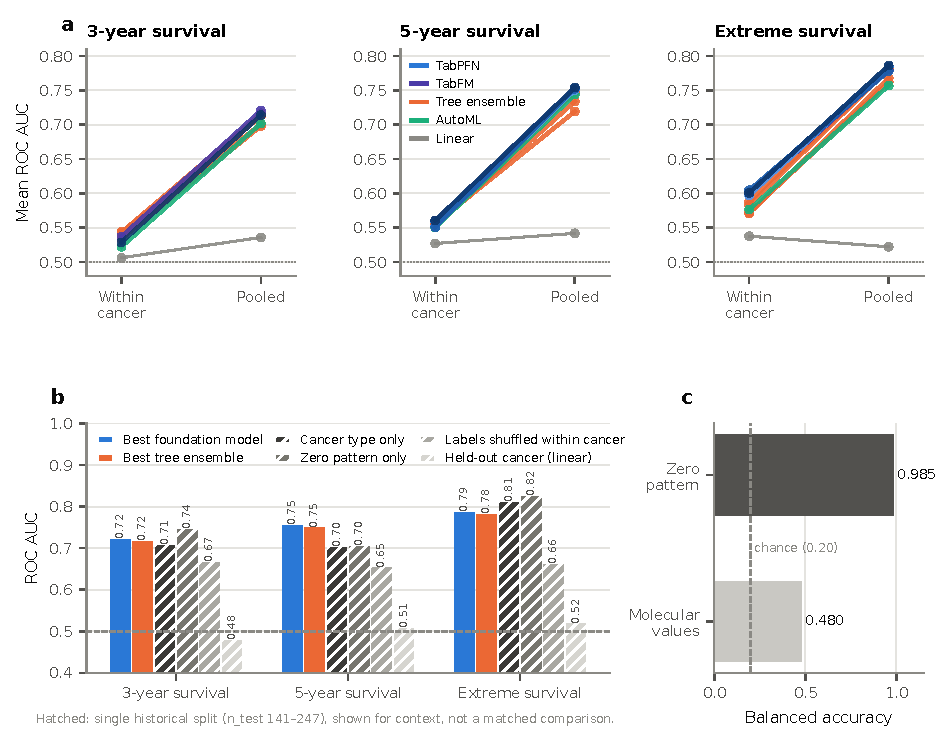
\includegraphics[width=\linewidth,height=0.64\textheight,keepaspectratio]{figures/reusability/fig4_pooling_and_controls.pdf}
\caption{\textbf{Pooling lifts every model, and controls without patient biology reach similar levels.} \textbf{a}, Mean ROC AUC within cancers and in the pooled cohort for each model, by endpoint; lines are coloured by model family. \textbf{b}, Pooled ROC AUC of the best foundation model and the best tree ensemble (solid bars; frozen benchmark) compared with four controls that ignore patient biology: cancer type only, zero pattern only, survival labels shuffled within each cancer (mean of 500 permutations) and a linear model tested on a held-out cancer (mean over held-out cancers). Hatched bars come from a single earlier split and are shown for context, not as a matched comparison. \textbf{c}, How well the cancer type itself can be recovered: balanced accuracy for identifying the cancer from the zero pattern or from molecular values; the dashed line marks chance (0.20 for five cancers).}
\label{fig:pooling}
\end{figure}

\begin{table}[ht]
\centering
\caption{Pooled shortcut and cancer-held-out diagnostics (ROC AUC). Controls were computed on a single earlier split; the best evaluated model is the frozen-benchmark mean for each endpoint. Structural zero denotes the zero-pattern control.}
\label{tab:shortcuts}
\footnotesize\setlength{\tabcolsep}{3pt}\begin{tabular}{lrrrr}
\toprule
Endpoint & Cancer identity & Structural zero & Best evaluated model & Held-out molecular \\
\midrule
3-year OS & 0.707 & 0.745 & 0.721 & 0.479 \\
5-year OS & 0.703 & 0.704 & 0.754 & 0.508 \\
Extreme OS & 0.809 & 0.824 & 0.786 & 0.518 \\
\bottomrule
\end{tabular}

\end{table}

\subsection*{Pooled training lowered within-cancer ranking for foundation models}

A clinician does not rank a breast cancer patient against a lung cancer patient; the diagnosis is already known. The comparison that matters is how well a model ranks patients who share a cancer. Every patient in a pooled task also appears in the corresponding cancer-specific task, so we compared, patient by patient, predictions from a model trained on that cancer alone with predictions from a model trained on the pooled cohort, scoring both only within the cancer.

Pooling did not significantly improve within-cancer ranking for any foundation model, and for several it made ranking worse (Fig.~\ref{fig:effect}a). At 5 years, pooled training lowered the within-cancer ROC AUC of TabFM from 0.540 to 0.456, a change of $-0.084$ (95\% CI, $-0.129$ to $-0.039$), and of TabPFN v3 from 0.539 to 0.469 ($-0.070$; $-0.114$ to $-0.027$). For extreme survival, TabFM fell by 0.081 ($-0.125$ to $-0.032$) and TabPFN v2.6 by 0.068 ($-0.112$ to $-0.023$). Tree ensembles showed smaller estimated changes, at most 0.04 in either direction, with every interval spanning zero. Cancer by cancer, the median change for foundation models was $-0.053$ at 5 years and $-0.036$ for extreme survival, against $-0.010$ and $+0.020$ for tree ensembles; at 3 years both medians were close to zero ($-0.011$ and $-0.020$; Fig.~\ref{fig:effect}b). The only intervals above zero belonged to the two weakest within-cancer models at 3 years, logistic regression ($+0.071$) and AutoGluon ($+0.073$). Of the 30 model--endpoint comparisons, four excluded zero in the negative direction, and all four were foundation models. Because some exclusions are expected by chance across 30 intervals, we place more weight on the direct comparison between families.

Averaged across models, foundation models lost more within-cancer ROC AUC than tree ensembles at every endpoint (Fig.~\ref{fig:effect}c): by 0.027 at 3 years (95\% CI, $-0.060$ to $0.005$), 0.030 at 5 years ($-0.065$ to $0.003$) and 0.042 for extreme survival ($-0.078$ to $-0.005$). Only the extreme-survival difference was resolved by its interval. The consistent direction, together with the four foundation-model exclusions, suggests that pooling degrades within-cancer ranking more for in-context models than for trees. The evidence is consistent but not conclusive.

\begin{figure}[tbp]
\centering
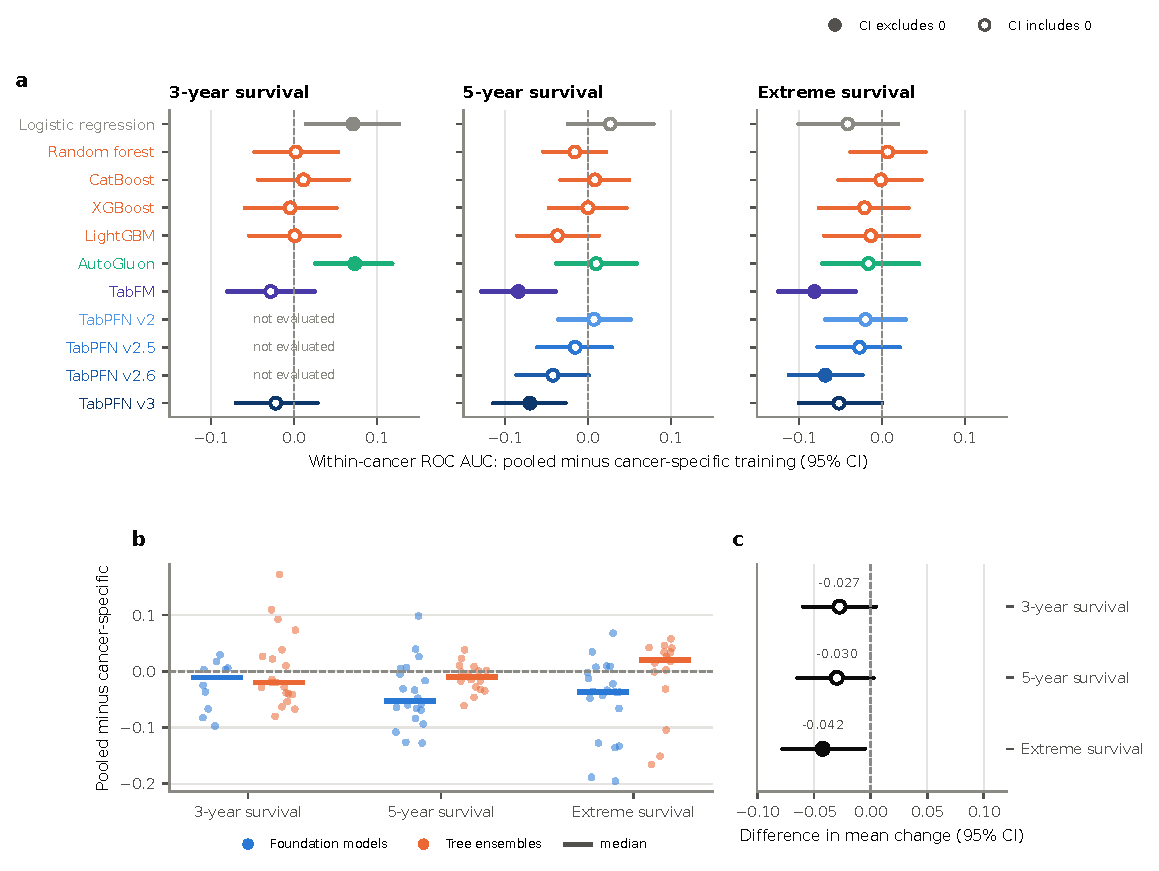
\includegraphics[width=\linewidth,height=0.64\textheight,keepaspectratio]{figures/reusability/fig5_within_cancer_effect.pdf}
\caption{\textbf{Pooled training lowered within-cancer ranking for foundation models.} \textbf{a}, For each model and endpoint, the mean across cancers of the within-cancer ROC AUC of the pooled model minus that of the cancer-specific model, scored on the same patients. Bars are 95\% patient-bootstrap intervals (2,000 resamples, shared across models); filled circles mark intervals that exclude zero. TabPFN v2--v2.6 were not evaluated on pooled 3-year survival. \textbf{b}, The same change shown cancer by cancer: each dot is one model in one cancer, grouped into foundation models and tree ensembles; horizontal bars mark medians. \textbf{c}, Foundation models minus trees: the mean change of foundation models minus that of tree ensembles at each endpoint, with its 95\% interval from the same resamples; a negative value means foundation models lost more.}
\label{fig:effect}
\end{figure}

\FloatBarrier

\section*{Discussion}

This report set out to test whether TabPFN's small-data advantage carries over to cancer survival prediction from multiomics. First, the direction of the original claim reproduced on TabPFN's own benchmark datasets under a simpler protocol: TabPFN had the highest mean ROC AUC among default-setting models, and its generations and TabFM were nearly interchangeable. Second, within single cancers, TabPFN remained competitive and was frequently the best model, but survival was hard for every method and no nonlinear model was significantly better than another. Third, pooling cancers raised every capable model by a similar margin (Fig.~\ref{fig:pooling}a), and controls without patient biology reached comparable scores (Fig.~\ref{fig:pooling}b). Fourth, pooled training lowered within-cancer ranking, more for the foundation models than for tree ensembles (Fig.~\ref{fig:effect}).

Our verdict is that TabPFN is reusable for the single-cohort, fixed-horizon survival tasks we studied. It runs without tuning, performed comparably to default-setting tree ensembles (a comparison that cannot establish equivalence), and had slightly lower log loss and Brier score than the tree ensembles in the pooled tasks (Extended Data Fig.~\ref{fig:ed_prob}), although neither measure establishes calibration.\citep{van2019calibration} This is in line with the independent clinical comparison, in which TabPFN's advantage over tuned established methods was inconsistent and generally within 0.02 AUROC.\citep{shaktah2026established} Our baselines were not tuned, and in large benchmarks tuning and ensembling can change rankings,\citep{erickson2025tabarena} so the comparison is between default settings. Its pooled pan-cancer scores, however, should not be read as patient-level prognosis.

We do not have a mechanistic account of why pooling hurt the foundation models more, and we offer one as a hypothesis to be tested. TabPFN attends across training samples and across features and fits no task-specific weights,\citep{hollmann2025accurate} and we hypothesise that its prediction for a patient therefore depends on the training rows most similar to that patient. We did not measure attention or run an ablation, so the architecture paper describes how the model computes and not why pooling hurt it. In the pooled table, the most similar rows are plausibly those from the same cohort, which the zero pattern identifies almost perfectly, and they share the cohort's average outcome. Tree ensembles build predictions from splits on individual features,\citep{breiman2001random,chen2016xgboost} which may make them less able to collapse onto a single latent variable. The hypothesis is directly testable. Standardizing features within each cancer and removing the zero fingerprint before pooling should restore within-cancer ranking for the foundation models if it is right, and should leave the gap unchanged if it is wrong; designs that add uninformative feature blocks or remove modalities have been used in a similar way to probe multiomics survival models.\citep{wissel2023systematic} This is the analogue of the remedies tested in previous reusability reports, and we have not yet run it.

Three bodies of work place the result in context without explaining it. In transfer learning, negative transfer is defined by comparison with learning on the target alone, which is the comparison in Fig.~\ref{fig:effect}, although that work concerns image domain adaptation and not in-context learning on pooled tables.\citep{wang2019characterizing} In prediction-model validation, discrimination depends on case mix, and an average over settings can conceal wide variation between them.\citep{dejong2023propensity,riley2016external} Our within-cancer scoring stratifies by cancer; it does not reweight patients to a target population, as propensity-based standardization does.\citep{dejong2023propensity} In routine health data, the presence or absence of a measurement can itself carry information, and models that exploit it can lose accuracy when the reason for missingness changes after deployment.\citep{sisk2021informative,rockenschaub2024robust} The zero pattern in our data records which assays were run for a cohort and not clinical behaviour, so these studies are analogies and not evidence about our mechanism. Finally, because TCGA molecular classes are organized largely by cell of origin,\citep{hoadley2018cell} the cohort information that models can use is partly biological, and the shortcut should not be dismissed as batch effect alone.

A reasonable counterargument is that, for an unselected pan-cancer population, cohort membership is part of the prediction problem. In oncology, though, the cancer type is known before any molecular profile is taken, so a pooled score answers a different question from the one asked at diagnosis. Within-cancer results answer the clinical question; pooled results, reported alone, can overstate it. Modest within-cancer discrimination is not unique to these models: in an 18-cohort TCGA benchmark, the best censored-survival method exceeded a clinical-variables-only reference by 0.002 to 0.028 in C-index in breast, head and neck, and both lung cancers, with the winning method chosen retrospectively in each cancer; C-index and ROC AUC are different measures and the values are not comparable.\citep{herrmann2021benchmark} The extreme-survival endpoint deserves the same caution. It produced the highest scores in the study but does not estimate performance for the fixed-horizon population, and its controls were the strongest of the three endpoints.

Using these models was straightforward. TabPFN and TabFM installed cleanly, needed no tuning, and ran on CPU. Three additions would make them easier to reuse in biomedical work. First, clear guidance on the 1,000-sample CPU safeguard of TabPFN v2 to v2.6, which excluded those versions from our largest task and is a runtime safeguard distinct from the models' recommended data sizes (for example 10,000 rows for TabPFN v2 and 50,000 for v2.5).\citep{hollmann2025accurate,priorlabs2025tabpfn25} Second, documented behavioral differences between generations, which our results suggest are small on public benchmarks but may matter under cohort structure. Third, a supported interface for censored time-to-event outcomes.

The limitations follow from the design. Fixed-horizon labels discard patients censored before the horizon, about half the cohort at 3 years. The reproduction used six datasets and one split each, raw ROC AUC and untuned baselines, whereas the original used 29 datasets, ten seeds and normalised scores, and we did not tabulate its per-dataset values. Clinical variables were excluded from our models, and survival benchmarks that include them use censored time-to-event metrics, so neither their results nor their conclusions about clinical-only references transfer directly to ours.\citep{herrmann2021benchmark,li2024combining} Cancer-specific test sets were small. The shortcut controls came from a single earlier split. The cancer-held-out diagnostic used a linear model with label-free feature selection that included the held-out cancer, and it was not repeated with foundation models; internal-external validation that leaves out one study at a time is the standard way to check transport across settings,\citep{riley2016external} and our diagnostic is a weaker version of it. The paired within-cancer analysis bootstraps patients, not model retraining. Finally, all data came from TCGA and CPTAC. The next steps are censored survival modeling applied identically to every model, the within-cancer standardization test described above, a comparison with clinical stage and age, and validation in an independent cohort. Until then, a pooled score is the beginning of an argument about biology, not its conclusion.

\section*{Methods}

\subsection*{Reproducibility experiments}
Seven classification datasets from the TabPFN benchmark suite were obtained from the public reproduction repository included in our project. For the baseline comparison, each dataset was split once into training and test partitions, stratified by class, with 15\% held out. TabPFN, CatBoost, XGBoost, LightGBM, random forest, logistic regression and AutoGluon were run with default settings. For the generation comparison, TabPFN v1, v2, v2.5, v2.6 and v3 and TabFM were evaluated with training sets capped at 1,024 rows by stratified subsampling. ROC AUC used one-vs-rest averaging for multiclass datasets. Runs that failed are reported as missing and not imputed.

\subsection*{Cancer cohorts and outcomes}
We used harmonized molecular and clinical data for BRCA, ESCA, HNSCC, LSCC and LUAD from the TCGA PanCancer Atlas and CPTAC proteogenomic studies.\citep{tcga2012brca,tcga2017esca,tcga2015hnsc,tcga2012lusc,tcga2014luad,liu2018clinical,li2023pancancer} Molecular features comprised RNA expression, copy number, DNA methylation and somatic mutation; clinical covariates were excluded from all models. For a horizon $h$ of 1,095 days (3 years) or 1,825 days (5 years), death on or before $h$ was labeled 1 and follow-up beyond $h$ was labeled 0; patients censored before $h$ were excluded. The extreme-survival endpoint compared death within 3 years with survival beyond 5 years.

\subsection*{Frozen evaluation}
Each task used five repeats of five patient-grouped outer folds, with about 20\% of patients in each test set and the remainder divided into training (about 64\% overall) and validation (about 16\%). All 400 test sets were frozen with checksums before any model was run. Pooled tasks were harmonized on exact shared feature identifiers, with features absent from a cohort set to zero. Within each fold, the 100 highest-variance molecular features were selected on training patients only, which avoids the selection bias that arises when features are chosen using all patients.\citep{ambroise2002selection} Validation patients were used only to choose a classification threshold.

\subsection*{Models}
We compared logistic regression, random forest, CatBoost, XGBoost, LightGBM, AutoGluon (180-second limit per fold), TabFM (PyTorch implementation) and TabPFN v2, v2.5, v2.6 and v3, all on CPU at default settings, with no hyperparameter tuning of any model, and seed 42.\citep{breiman2001random,chen2016xgboost,ke2017lightgbm,prokhorenkova2018catboost,erickson2020autogluon,hollmann2025accurate,google2026tabfm,tabfmsoftware2026} AutoGluon's 180-second limit is far shorter than the one- to four-hour budgets of its original benchmark.\citep{erickson2020autogluon} TabPFN-3 was run from the local checkpoint, and hosted-API variants were not evaluated.\citep{priorlabs2026tabpfn3} TabFM is documented in a Google announcement and a software repository. Model code was taken from the TabPFN repository at commit \texttt{c0bc41a}, the TabPFN-3 checkpoint repository at commit \texttt{2997265} and the TabFM repository at commit \texttt{5ee6cd7}. TabPFN v2 to v2.6 refuse CPU inference with more than 1,000 training samples by default, a runtime safeguard and not their recommended data size, so the pooled 3-year task (about 1,050 training patients) was not evaluated for those versions.
% TODO before submission: add exact package versions (pip freeze of the evaluation image and local environment).

\subsection*{Metrics and statistics}
ROC AUC was the primary measure; precision-recall AUC, log loss, Brier score and threshold-dependent metrics were also recorded. Precision-recall AUC depends on event prevalence and was read against it,\citep{saito2015precision} and a lower log loss or Brier score\citep{brier1950verification} indicates better aggregate probability estimates without establishing calibration.\citep{van2019calibration} We use two ROC AUC summaries and name them distinctly. Fold-mean AUC is the mean over the 25 test sets of a task (Tables~\ref{tab:model_auc} and~\ref{tab:shortcuts}, Figs.~\ref{fig:within} and~\ref{fig:pooling}a). Patient-averaged within-cancer AUC is computed after averaging each patient's test predictions across the five repeats (Fig.~\ref{fig:effect}). Models were compared across the 13 cancer-specific tasks with the Friedman test on per-task mean AUC and the Nemenyi critical difference for $k = 11$ models;\citep{demsar2006statistical} non-significance was not treated as equivalence.

\subsection*{Controls}
On a single earlier split of each pooled cohort, the cancer-type control was a logistic model whose only input was cancer type. The zero-pattern control used a binary indicator of whether each selected feature was zero or missing. Cohort identifiability was estimated by predicting cancer type from molecular values or from the zero pattern. Label-permutation nulls used 500 permutations per endpoint, either across all patients or within each cancer. In the cancer-held-out diagnostic, a linear molecular model was trained on all but one cancer and tested on the omitted one, with features preselected without labels in the pooled cohort.

\subsection*{Paired within-cancer comparison}
For each model and endpoint, we averaged each patient's test probability across repeats separately for the cancer-specific and the pooled model, computed the ROC AUC of each within every cancer, and took the difference. Uncertainty came from 2,000 bootstrap resamples of patients, stratified by outcome within each cancer and shared across models so that differences between model families are paired. The family comparison is the mean change of foundation models (TabFM and the TabPFN versions evaluated at that endpoint) minus the mean change of tree ensembles (random forest, CatBoost, XGBoost and LightGBM), with a 95\% percentile interval.

\subsection*{Reproducibility of this report}
All figures and tables were generated from saved predictions and metrics; no model was refitted to produce them and no curve or interval was entered by hand. The scripts are \path{paper/analysis/reusability/compute_reusability_statistics.py} and \path{paper/analysis/reusability/build_reusability_figures.py} for the main figures, \path{paper/analysis/build_manuscript_assets.py} for tables and Extended Data, and \path{paper/analysis/within_cancer_pooling_contrast.py}. We consulted TRIPOD+AI for reporting and PROBAST+AI for risk of bias and applicability, but did not complete formal checklists.\citep{tripodai2024,probastai2024}

\section*{Data availability}
TCGA and CPTAC data are available from their originating resources under their terms of use. Frozen fold bundles are held in the Hugging Face dataset \path{TABR1-Cancer-OS-LeakageSafe-Folds} under the \path{HawkFranklin-Research} organization. Source data for every figure panel are provided in \path{paper/figures/reusability/source_data} and \path{paper/figures/source_data}.

\section*{Code availability}
All code is available at \url{https://github.com/HawkFranklin-Research/tab-r1}.

\section*{Author contributions}
V.P.P. and S.P.M. conceived the study. S.P.M. and V.P.P. performed the reproduction experiments; V.P.P. performed the cancer evaluation and analysis. Both authors interpreted the results and wrote the manuscript. Language-model assistance was used for code development, editing and reproducibility checks under human supervision; such tools are not authors and bear no responsibility for the conclusions.

\section*{Competing interests}
The authors declare no competing interests.

\bibliography{references}
\clearpage
\begingroup
\setcounter{figure}{0}
\renewcommand{\figurename}{Extended Data Fig.}
\renewcommand{\theHfigure}{extended.\arabic{figure}}

\begin{figure}[p]
\section*{Extended Data}
\centering
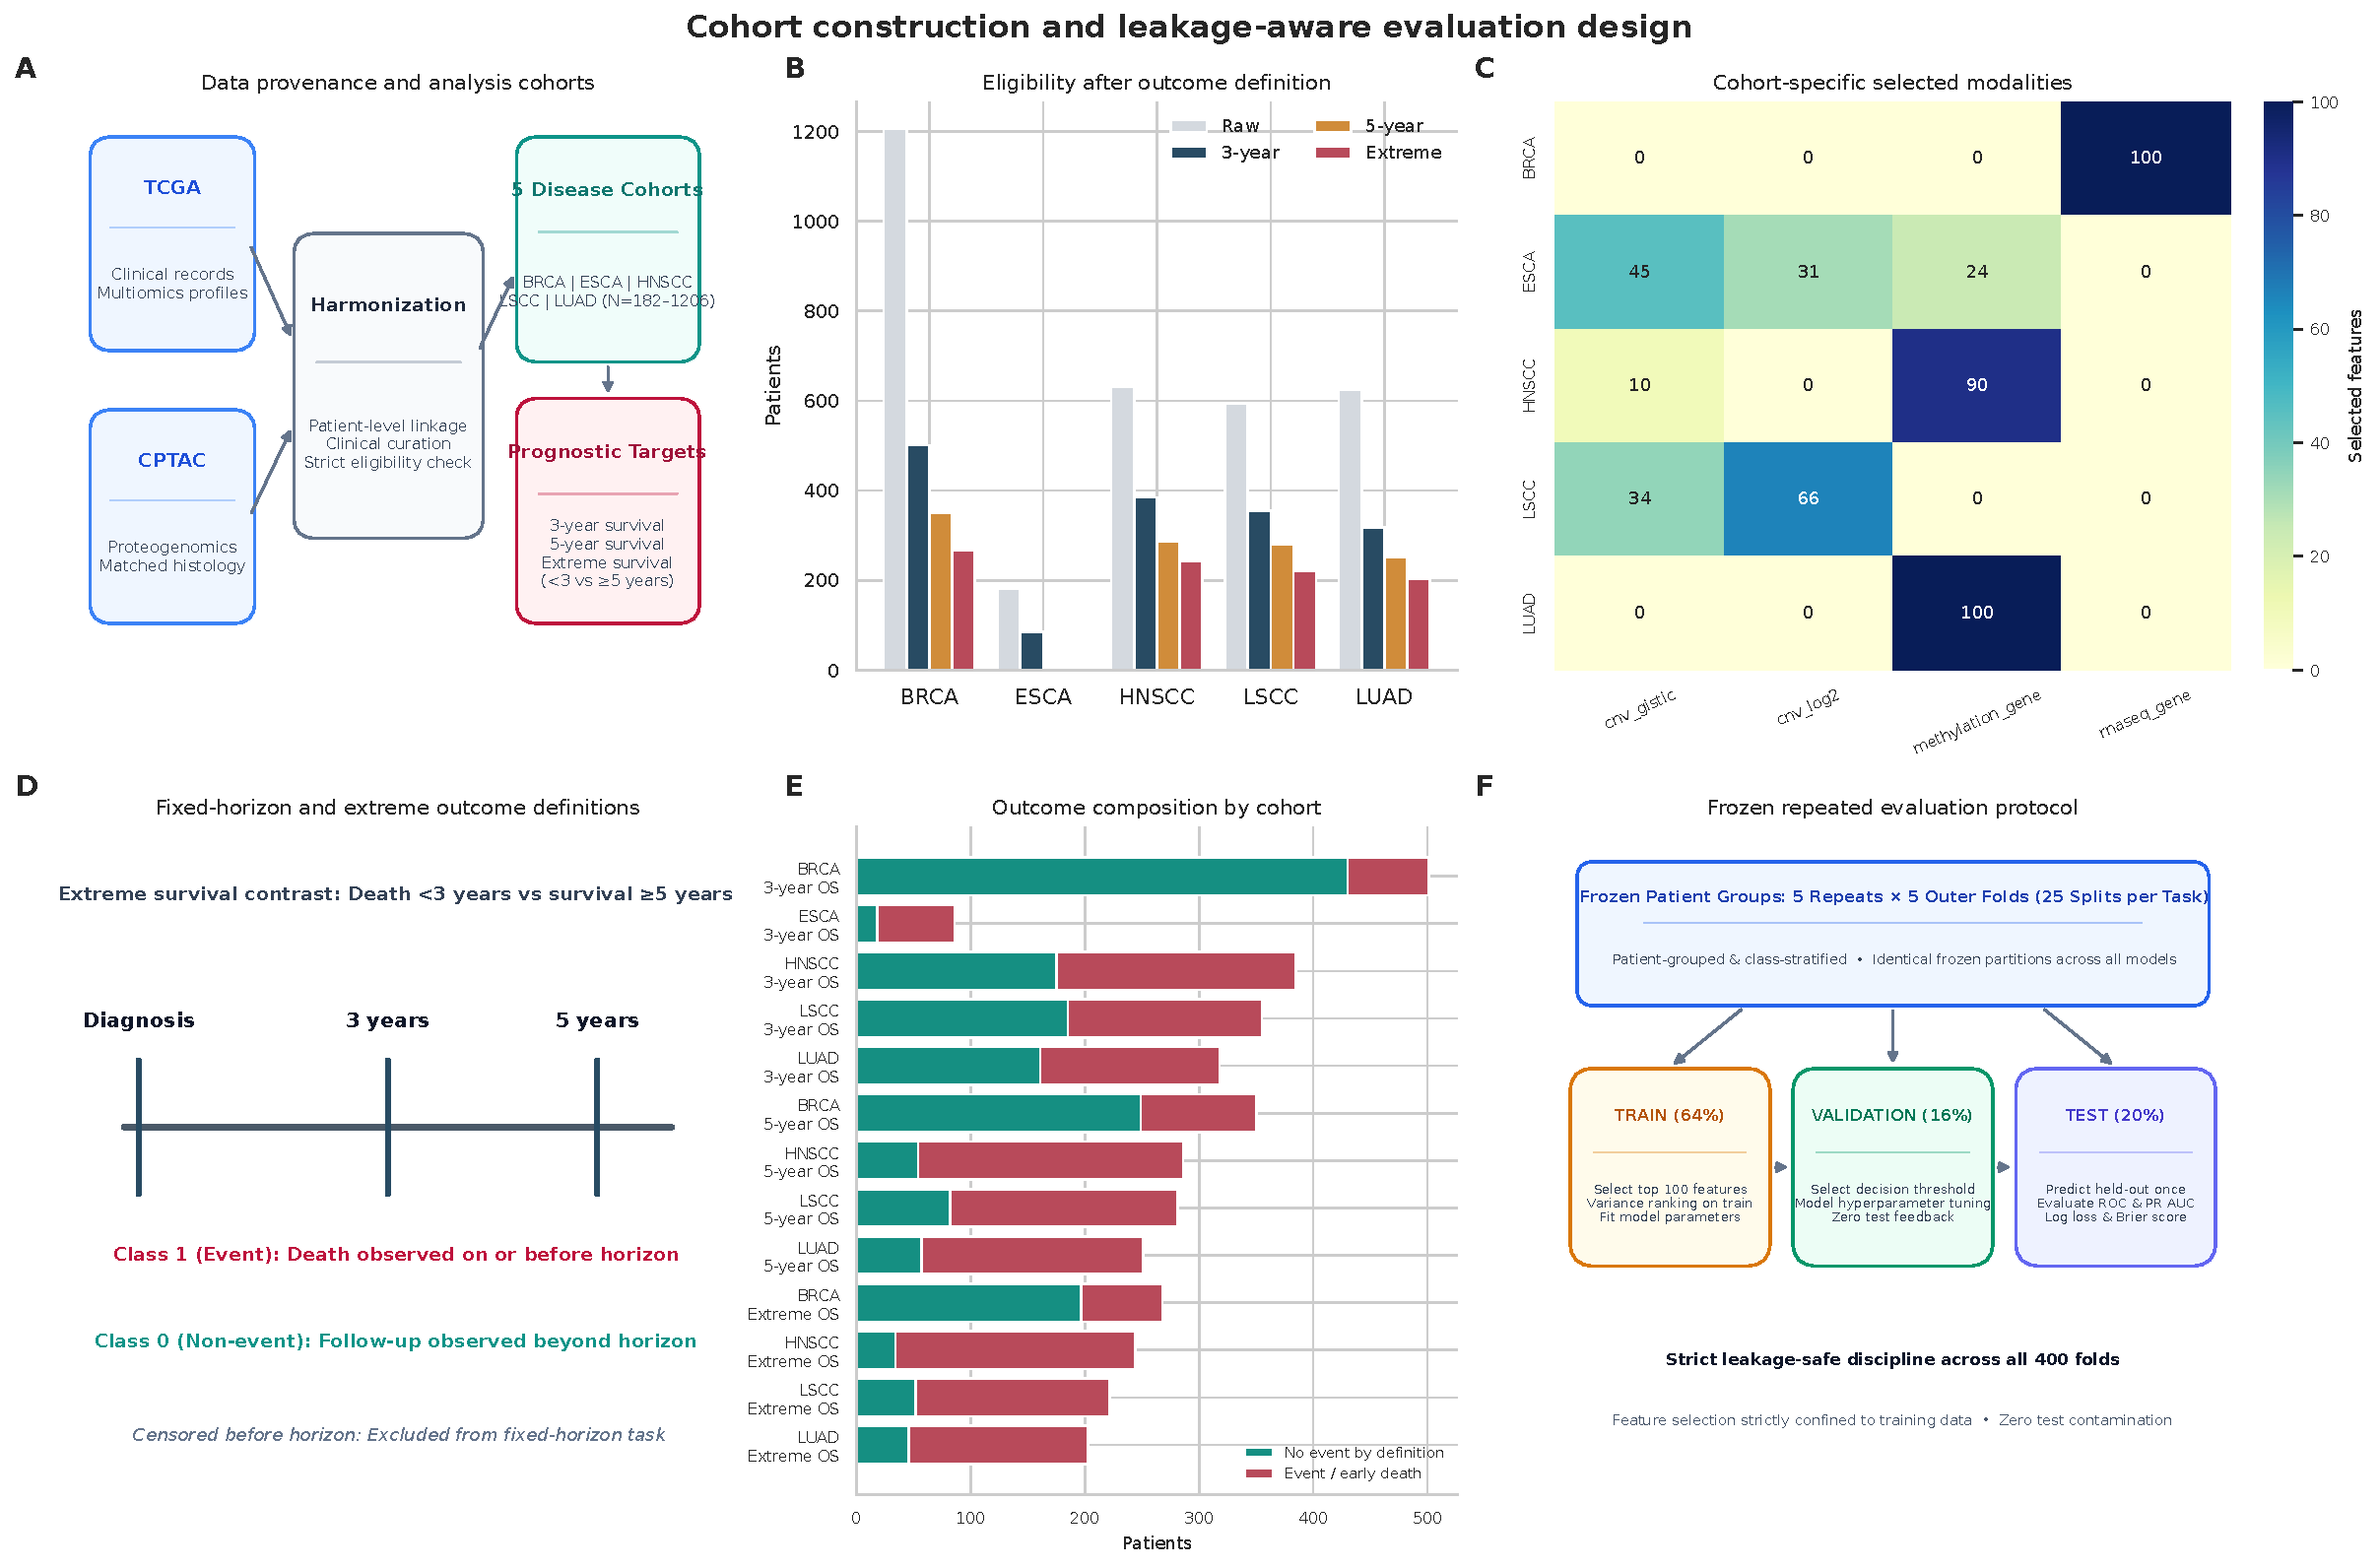
\includegraphics[width=\linewidth,height=0.64\textheight,keepaspectratio]{figures/manuscript/figure_01_cohort_and_design.pdf}
\caption{\textbf{Cohort detail.} Provenance, eligibility, molecular modality composition, endpoint definitions, class counts and the evaluation protocol for the five cohorts.}
\label{fig:ed_cohort}
\end{figure}

\begin{figure}[p]
\centering
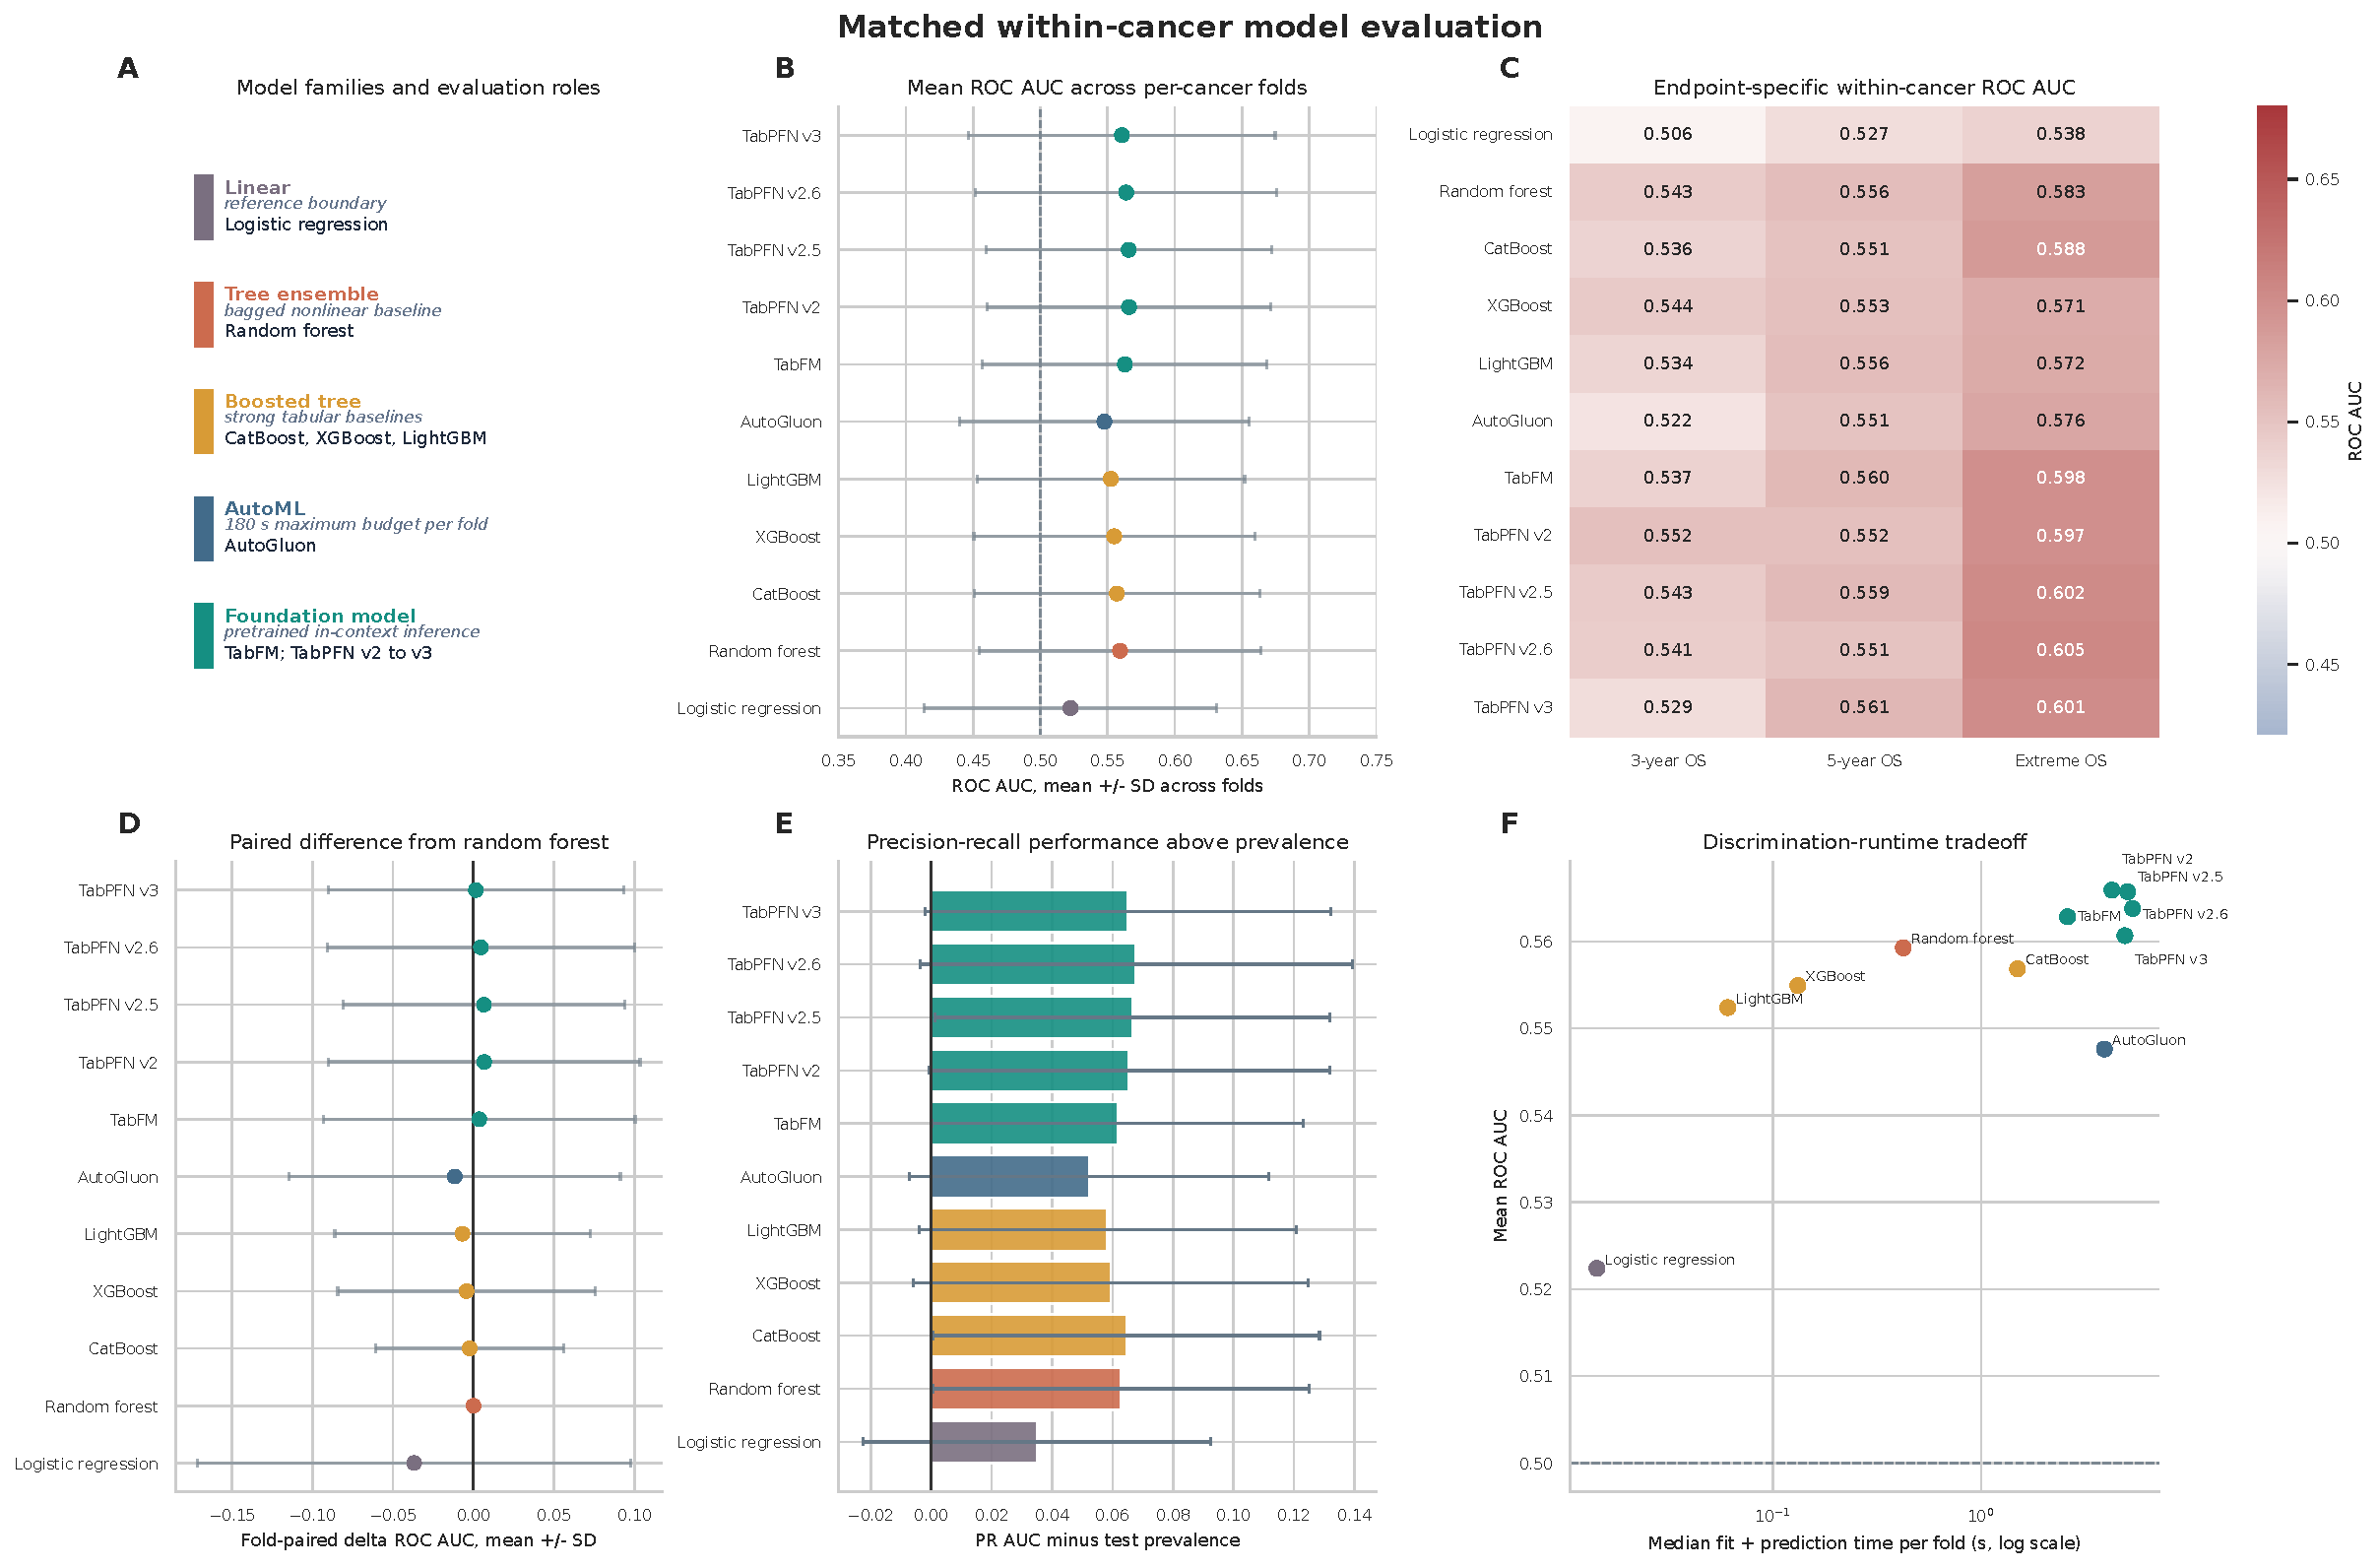
\includegraphics[width=\linewidth,height=0.64\textheight,keepaspectratio]{figures/manuscript/figure_02_within_cancer_performance.pdf}
\caption{\textbf{Within-cancer performance detail.} Model families, mean ROC AUC with variation across test sets, AUC by model and endpoint, fold-matched differences from random forest, precision-recall AUC above prevalence, and runtime.}
\label{fig:ed_within}
\end{figure}

\begin{figure}[p]
\centering
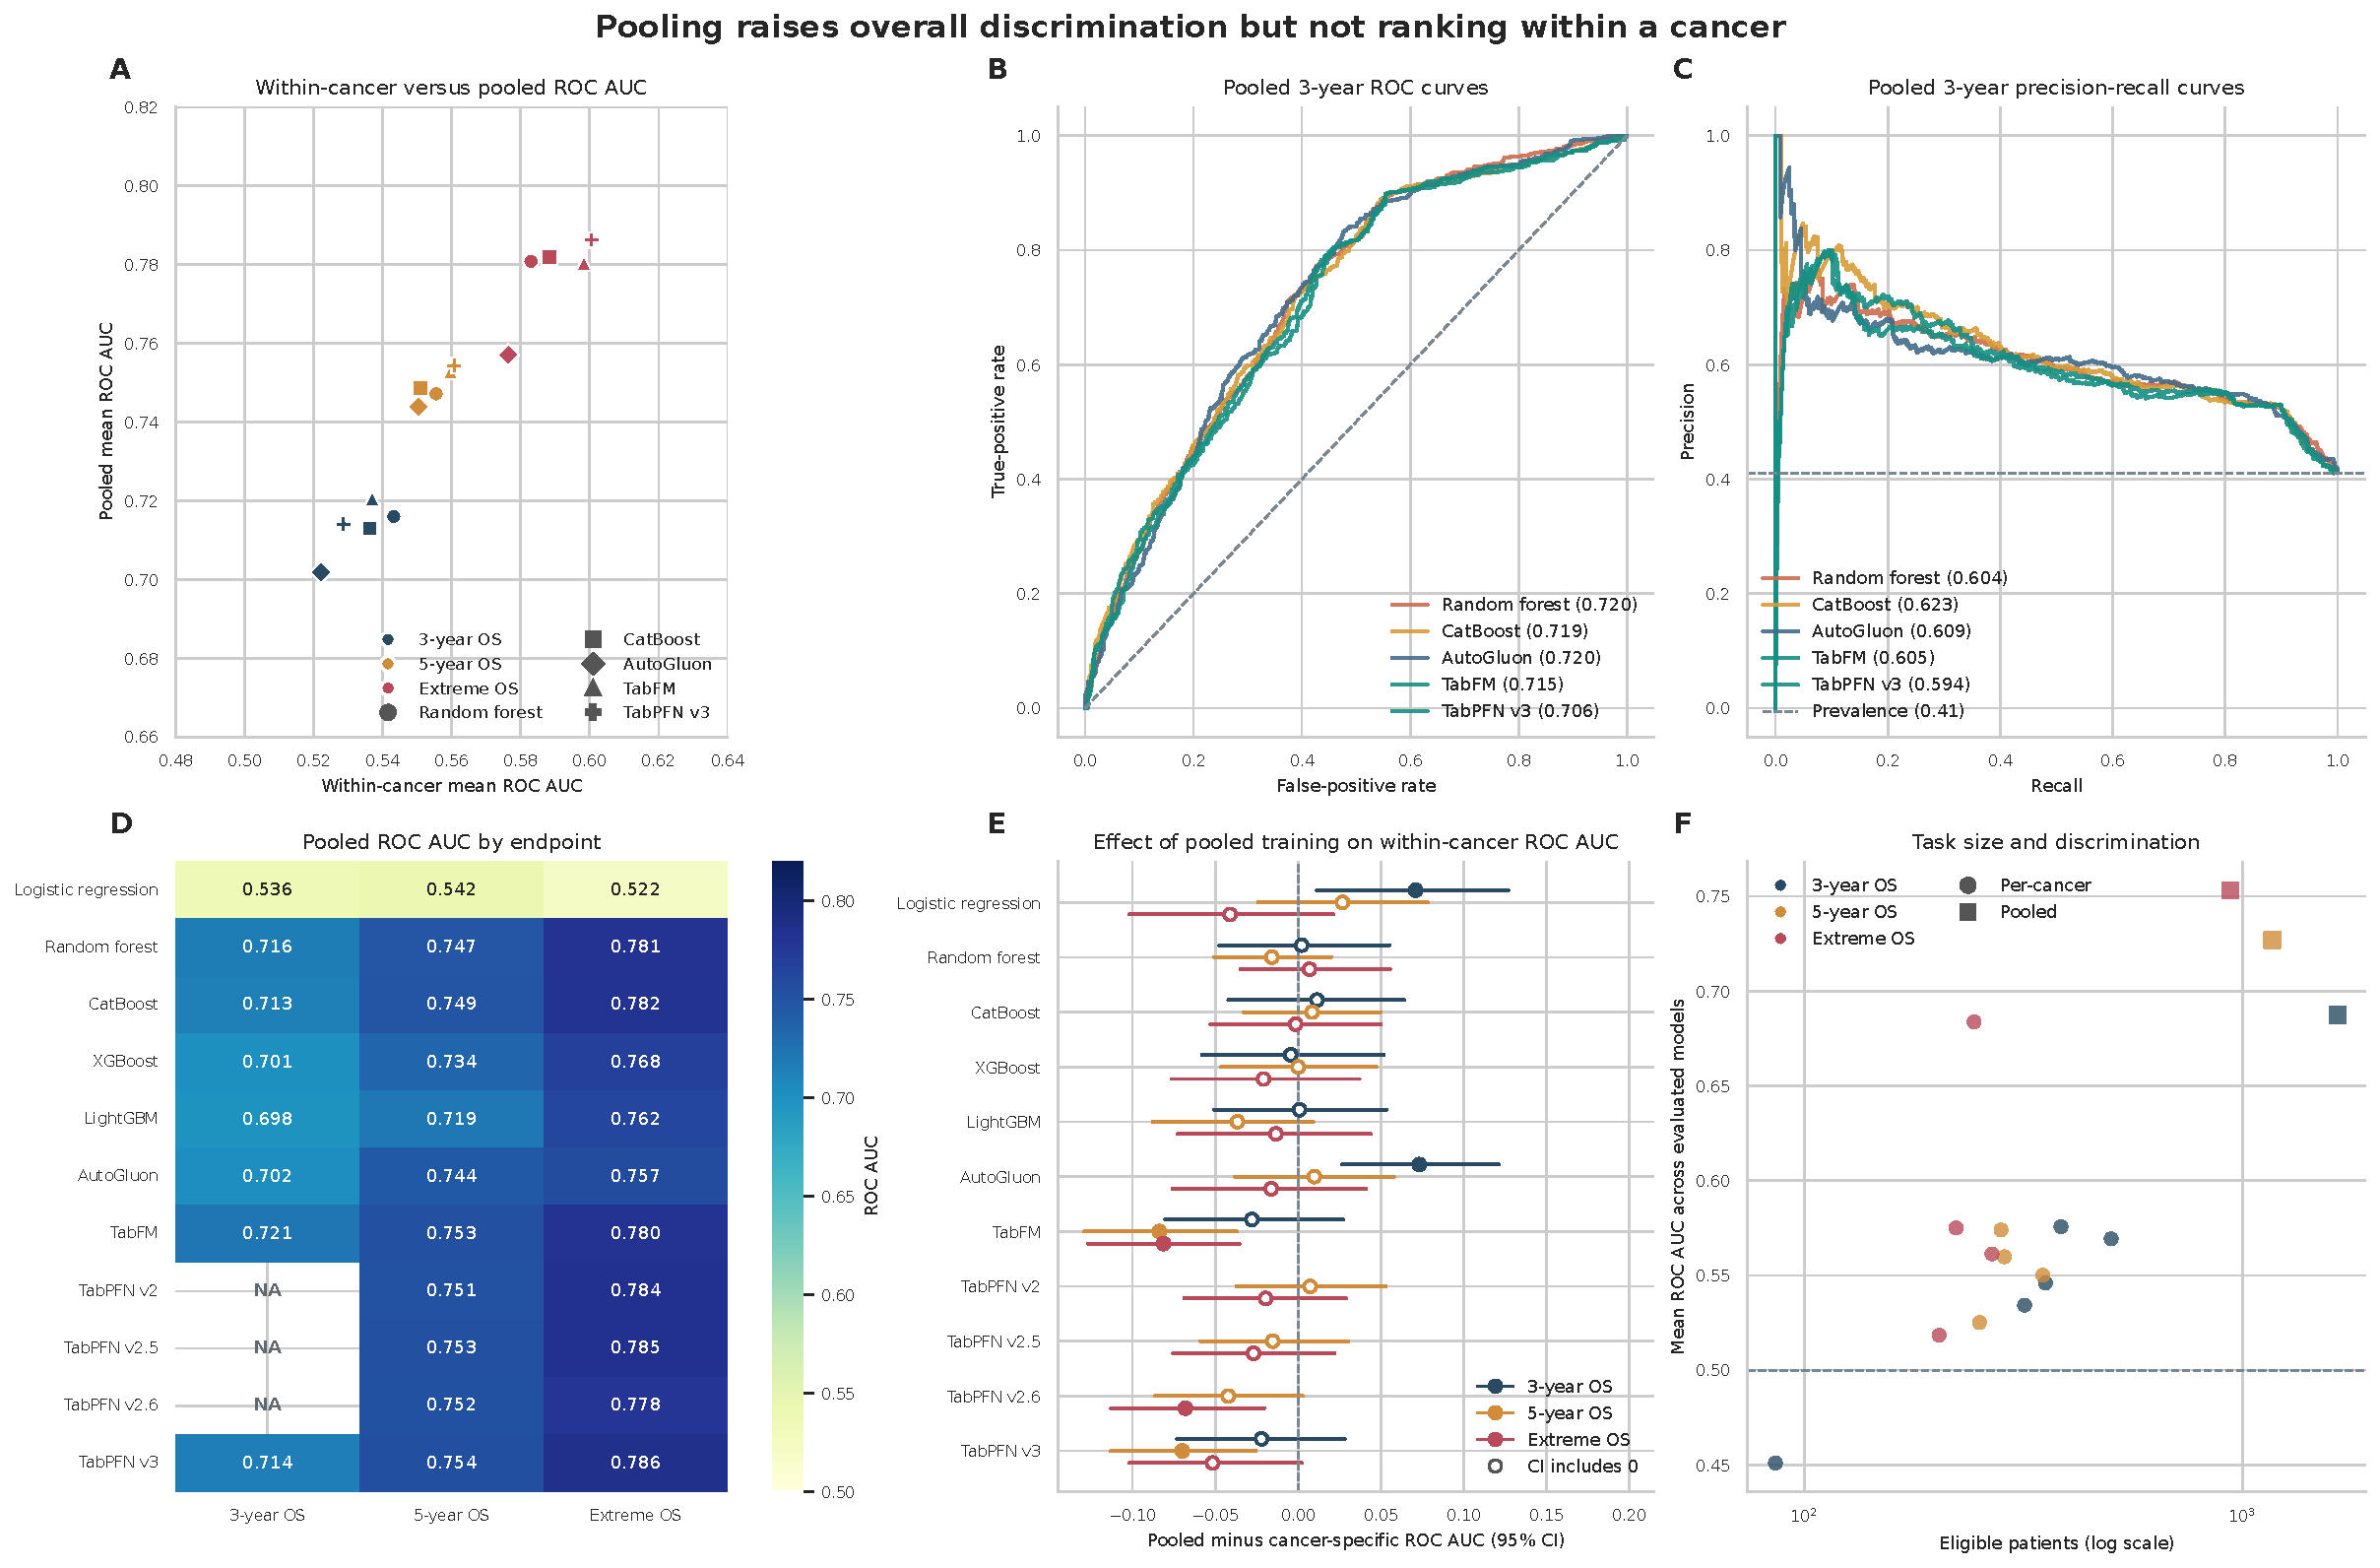
\includegraphics[width=\linewidth,height=0.64\textheight,keepaspectratio]{figures/manuscript/figure_03_pooling_effect.pdf}
\caption{\textbf{Pooled-task curves.} Within-cancer versus pooled AUC, pooled 3-year ROC and precision-recall curves, pooled AUC heatmap, the paired within-cancer effect (first version) and task size against discrimination.}
\label{fig:ed_pool}
\end{figure}

\begin{figure}[p]
\centering
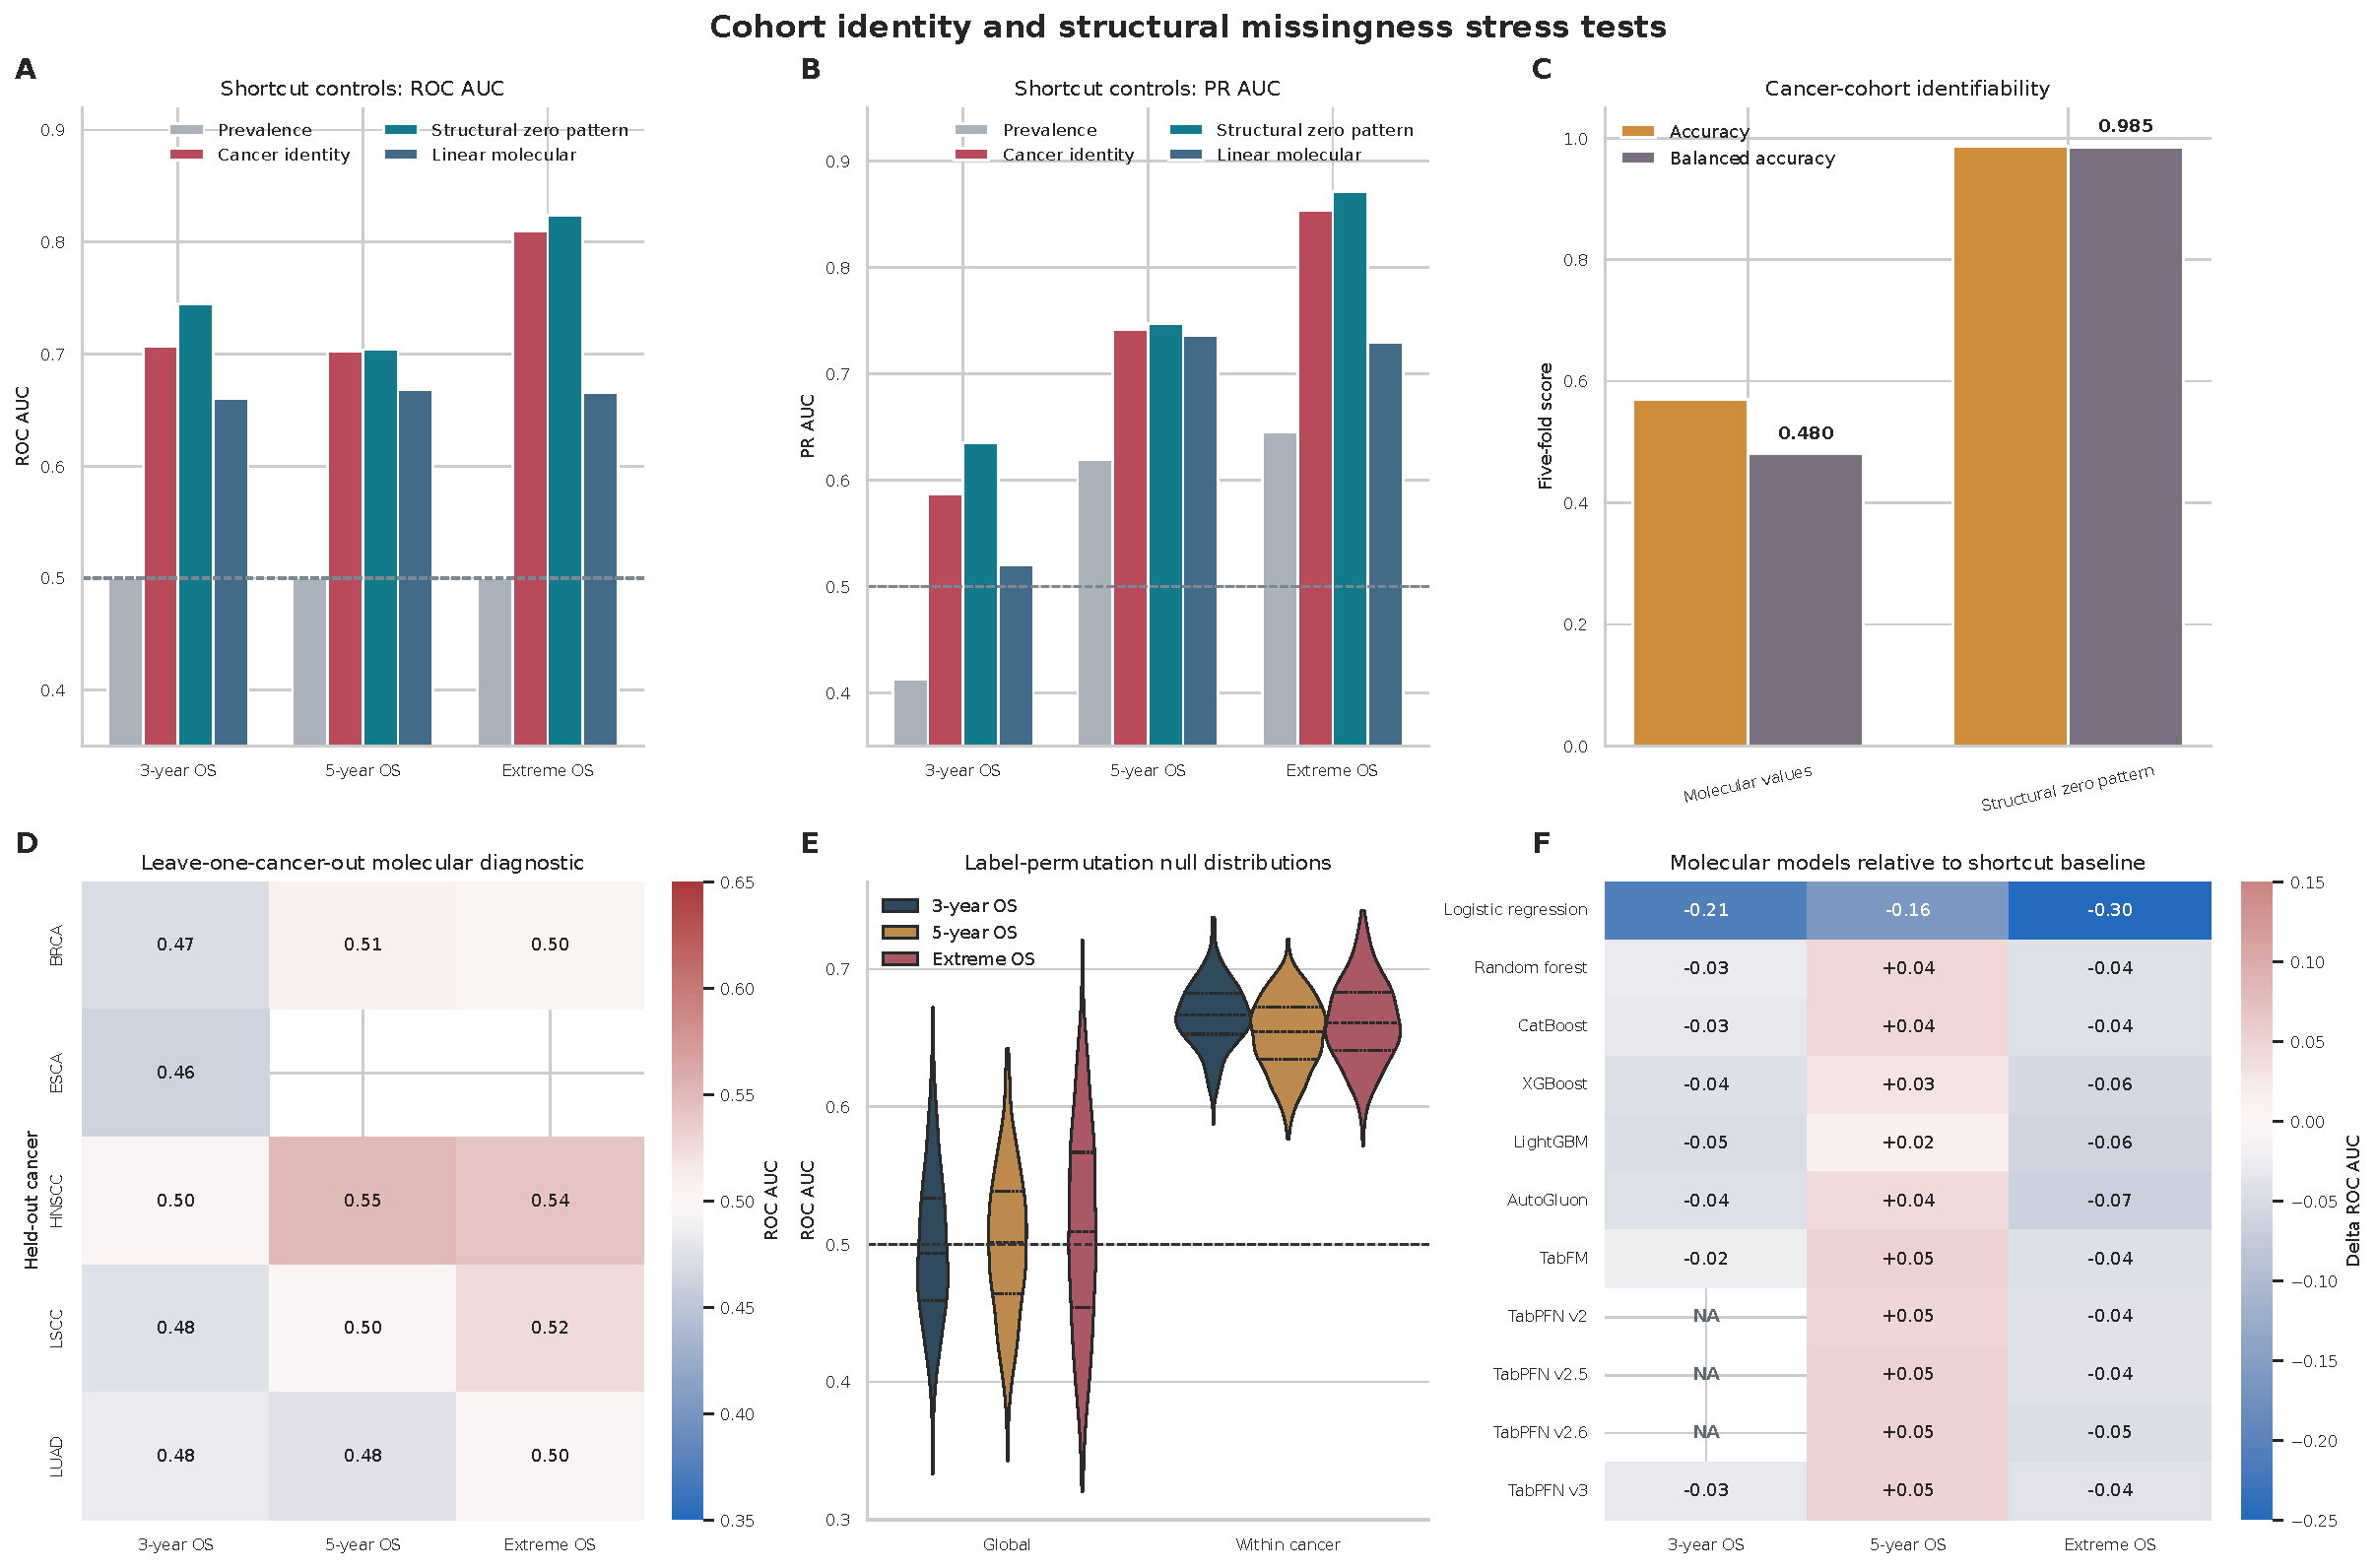
\includegraphics[width=\linewidth,height=0.64\textheight,keepaspectratio]{figures/manuscript/figure_04_shortcut_stress_tests.pdf}
\caption{\textbf{Shortcut-control detail.} Cancer-type and zero-pattern controls, cohort identifiability, cancer-held-out diagnostics, permutation distributions and the difference between each pooled model and the strongest control.}
\label{fig:ed_shortcut}
\end{figure}

\begin{figure}[p]
\centering
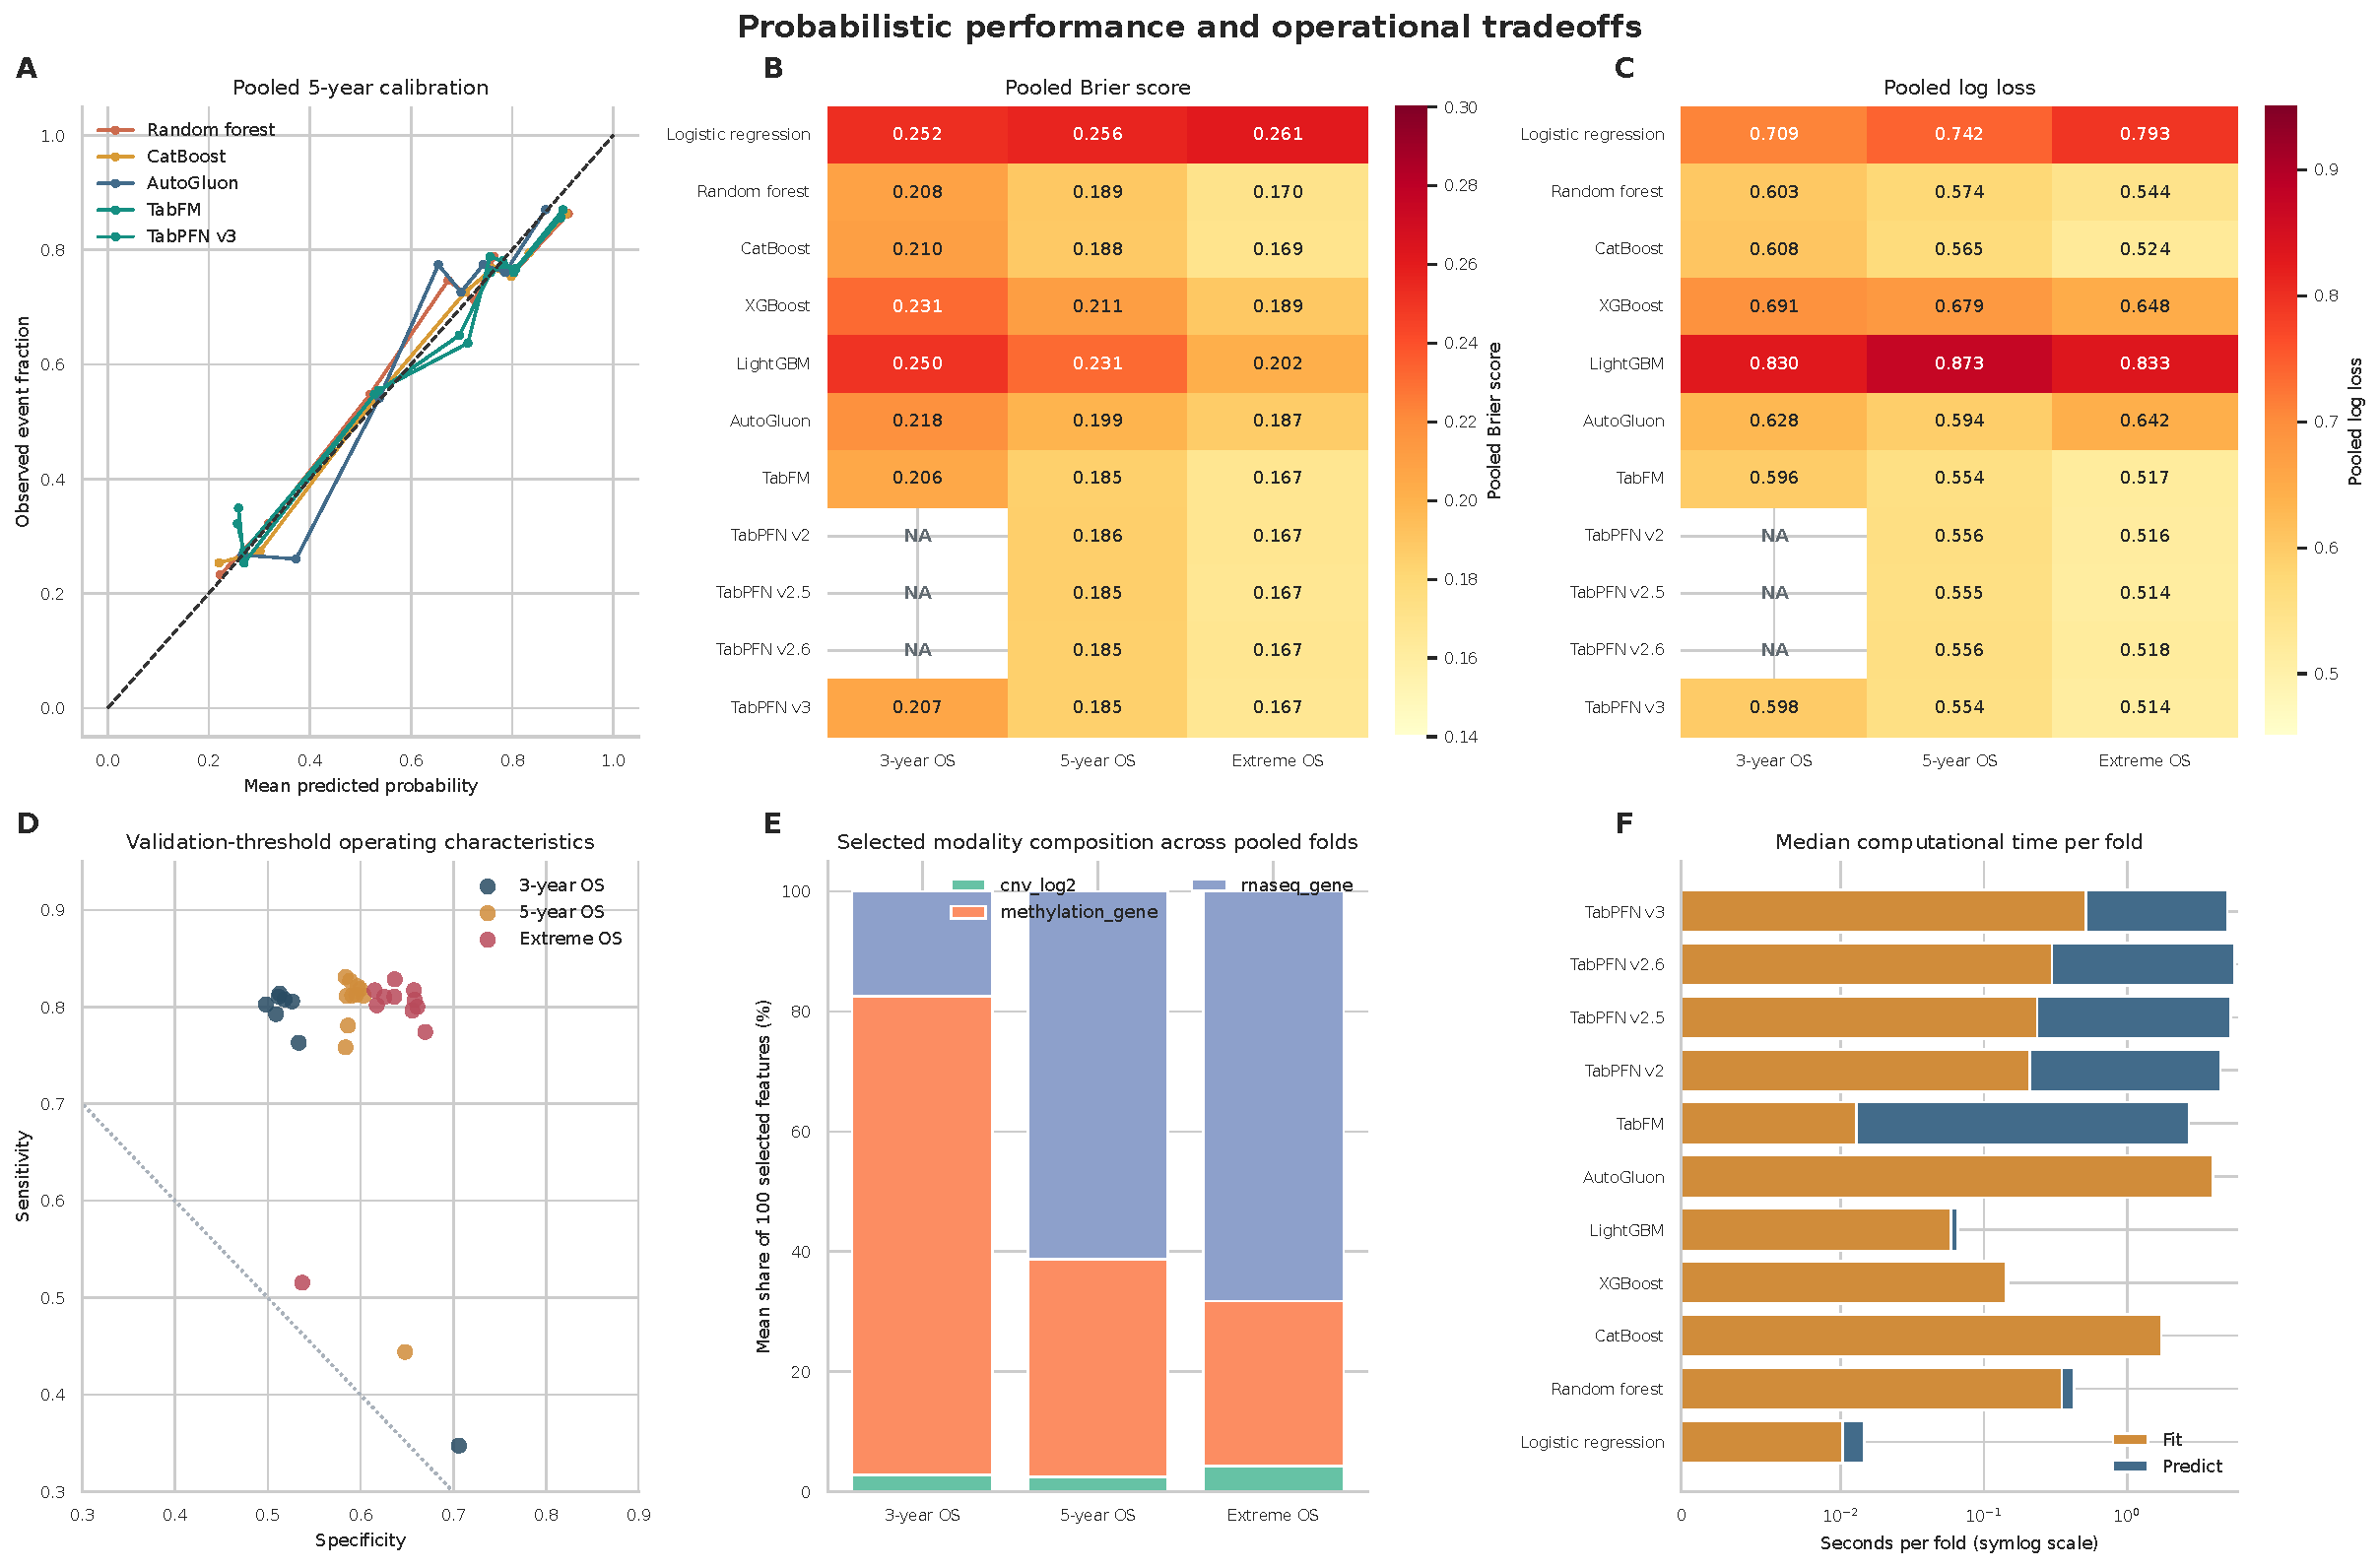
\includegraphics[width=\linewidth,height=0.64\textheight,keepaspectratio]{figures/manuscript/figure_05_probabilistic_and_compute.pdf}
\caption{\textbf{Probability quality and compute.} Calibration curves for pooled 5-year predictions, pooled Brier score and log loss, sensitivity and specificity at validation-selected thresholds, selected-feature modality composition, and median fit and prediction time per fold. Classical models ran locally and foundation models on a separate CPU machine, so runtimes are indicative.}
\label{fig:ed_prob}
\end{figure}


\endgroup

\end{document}
